%%%%%%%%%%%%%%%%%%%%%%%%%%%%%%%%%%%%%%%%%%%%%%%%%%%%%%%%%%%%%%%%
%
%  Template for homework of Introduction to Machine Learning.
%
%  Fill in your name, lecture number, lecture date and body
%  of homework as indicated below.
%
%%%%%%%%%%%%%%%%%%%%%%%%%%%%%%%%%%%%%%%%%%%%%%%%%%%%%%%%%%%%%%%%


\documentclass[11pt,letter,notitlepage]{article}
%Mise en page
\usepackage[left=2cm, right=2cm, lines=45, top=0.8in, bottom=0.7in]{geometry}
\usepackage{fancyhdr}
\usepackage{fancybox}
\usepackage{graphicx}
\usepackage{pdfpages} 
\renewcommand{\headrulewidth}{1.5pt}
\renewcommand{\footrulewidth}{1.5pt}
\newcommand\Loadedframemethod{TikZ}
\usepackage[framemethod=\Loadedframemethod]{mdframed}

\usepackage{amssymb,amsmath}
\usepackage{amsthm}
\usepackage{thmtools}
\newtheorem{definition}{Definition}

\usepackage{algorithm}
\usepackage{algorithmic}
% \usepackage[ruled]{algorithm2e}

\usepackage{ctex}
\usepackage{afterpage}
%%%%%%%%%%%%%%%%%%%%%%%%
%%%%%% Define math operator %%%%%
%%%%%%%%%%%%%%%%%%%%%%%%
\DeclareMathOperator*{\softmax}{\bf softmax}
\DeclareMathOperator*{\argmin}{\bf argmin}
\DeclareMathOperator*{\argmax}{\bf argmax}
\DeclareMathOperator*{\relint}{\bf relint\,}
\DeclareMathOperator*{\dom}{\bf dom\,}
\DeclareMathOperator*{\intp}{\bf int\,}
%%%%%%%%%%%%%%%%%%%%%%%

\addtocounter{MaxMatrixCols}{11}

\setlength{\topmargin}{0pt}
\setlength{\textheight}{9in}
\setlength{\headheight}{0pt}

\setlength{\oddsidemargin}{0.25in}
\setlength{\textwidth}{6in}
\pagestyle{fancy}
%%%%%%%%%%%%%%%%%%%%%%%%
%% Define the Exercise environment %%
%%%%%%%%%%%%%%%%%%%%%%%%
\mdtheorem[
topline=false,
rightline=false,
leftline=false,
bottomline=false,
leftmargin=-10,
rightmargin=-10
]{exercise}{\textbf{Exercise}}
%%%%%%%%%%%%%%%%%%%%%%%
%% End of the Exercise environment %%
%%%%%%%%%%%%%%%%%%%%%%%

%%%%%%%%%%%%%%%%%%%%%%%
%% Define the Solution Environment %%
%%%%%%%%%%%%%%%%%%%%%%%
\declaretheoremstyle
[
spaceabove=0pt, 
spacebelow=0pt, 
headfont=\normalfont\bfseries,
notefont=\mdseries, 
notebraces={(}{)}, 
headpunct={:\quad}, 
headindent={},
postheadspace={ }, 
postheadspace=4pt, 
bodyfont=\normalfont, 
qed=$\blacksquare$,
preheadhook={\begin{mdframed}[style=myframedstyle]},
	postfoothook=\end{mdframed},
]{mystyle}

\declaretheorem[style=mystyle,title=Solution,numbered=no]{solution}
\mdfdefinestyle{myframedstyle}{%
	topline=false,
	rightline=false,
	leftline=false,
	bottomline=false,
	skipabove=-6ex,
	leftmargin=-10,
	rightmargin=-10}
%%%%%%%%%%%%%%%%%%%%%%%
%% End of the Solution environment %%
%%%%%%%%%%%%%%%%%%%%%%%

%% Homework info.
\newcommand{\posted}{\text{Dec. 9, 2019}}       			%%% FILL IN POST DATE HERE
\newcommand{\due}{\text{Dec. 23, 2019}} 			%%% FILL IN Due DATE HERE
\newcommand{\hwno}{\text{7}} 		           			%%% FILL IN LECTURE NUMBER HERE


\newcommand{\expect}[1]{\text{E} [#1]}
\newcommand{\var}[1]{\text{Var} [#1]}

%%%%%%%%%%%%%%%%%%%%
%% Put your information here %%
%%%%%%%%%%%%%%%%%%%
\newcommand{\name}{\text{Jiahuan Yu}}  	          			%%% FILL IN YOUR NAME HERE
\newcommand{\id}{\text{PB17121687}}		       			%%% FILL IN YOUR ID HERE
%%%%%%%%%%%%%%%%%%%%
%% End of the student's info %%
%%%%%%%%%%%%%%%%%%%


\lhead{
	\textbf{\name}
}
\rhead{
	\textbf{\id}
}
\chead{\textbf{
		Homework \hwno
}}


\begin{document}
\vspace*{-4\baselineskip}
\thispagestyle{empty}


\begin{center}
	{\bf\large Introduction to Machine Learning}\\
	{Fall 2019}\\
	University of Science and Technology of China
\end{center}

\noindent
Lecturer: Jie Wang  			 %%% FILL IN LECTURER HERE
\hfill
Homework \hwno
\\
Posted: \posted
\hfill
Due: \due
\\
Name: \name
\hfill
ID: \id
\hfill

\noindent
\rule{\textwidth}{2pt}

\medskip





%%%%%%%%%%%%%%%%%%%%%%%%%%%%%%%%%%%%%%%%%%%%%%%%%%%%%%%%%%%%%%%%
%% BODY OF HOMEWORK GOES HERE
%%%%%%%%%%%%%%%%%%%%%%%%%%%%%%%%%%%%%%%%%%%%%%%%%%%%%%%%%%%%%%%%

\textbf{Notice, }to get the full credits, please present your solutions step by step.

\begin{exercise}[Properties of expectation and variance  \textnormal{10pts}]
	Let $X, Y,$ and $Z$ be random variables. Show that the following results hold.
	\begin{enumerate}
		\item (5pts) The tower property holds, i.e.,
		      \begin{align*}
			      \expect{X|Y} = \expect{ \expect{X|Y,Z} |Y}.
		      \end{align*}
		\item (5pts) The variance decomposition formula holds, i.e.,
		      \begin{align*}
			      \var{X} = \expect{\var{X|Y}}+\var{\expect{X|Y}}.
		      \end{align*}
	\end{enumerate}
	\emph{Hint: if you do not know measure theory well, you can assume that $X$, $Y$, and $Z$ are continuous random variables.}
\end{exercise}

\begin{solution}
	\begin{enumerate}
		\item 设 $X$ 的概率密度函数为 $$f(x;w,y,z)$$
		      则 $$\expect {X|Y=y}=\int_{w} \int_{z} f(x;w,y,z) \mathrm{d}z \mathrm{d}w $$
		      $$\begin{aligned}
				      \expect{ \expect{X|Y=y,Z=z} |Y=y}
				       & = \expect{ \int_{w} f(x;w,y,z) \mathrm{d}w |Y=y}                      \\
				       & = \int_{z} \left( \int_{w} f(x;w,y,z) \mathrm{d}w \right) \mathrm{d}z \\
				       & =\int_{w} \int_{z} f(x;w,y,z) \mathrm{d}z \mathrm{d}w
			      \end{aligned}$$
		      所以有 $$\expect{X|Y} = \expect{ \expect{X|Y,Z} |Y}$$
		\item 令上述证明中 $X$ 的概率密度为 $$f(x;w,z)$$
		      即可得到 $$\expect{X} = \expect{ \expect{X|Z}}$$
		      所以
		      $$\begin{aligned}
				        & \expect{\var{X|Y}}+\var{\expect{X|Y}}                                           \\
				      = & \expect{ \expect{X^2|Y}-\left( \expect{X|Y} \right)^2 }
				      + \expect{ \left( \expect{X|Y} \right)^2} - \left( \expect{ \expect{X|Z}} \right)^2 \\
				      = & \expect{ \expect{X^2|Y} }- \expect{\left( \expect{X|Y} \right)^2 }
				      + \expect{ \left( \expect{X|Y} \right)^2} - \left( \expect{ \expect{X|Z}} \right)^2 \\
				      = & \expect{ X^2 }- \expect{\left( \expect{X|Y} \right)^2 }
				      + \expect{ \left( \expect{X|Y} \right)^2} - \left( \expect{X} \right)^2             \\
				      = & \expect{ X^2 }- \left( \expect{X} \right)^2                                     \\
				      = & \var{X}
			      \end{aligned}$$
	\end{enumerate}
\end{solution}


\newpage
\begin{exercise}[Properties of transition matrix \textnormal{30pts}]
	A matrix is nonnegative (positive) if all its entries are nonnegative (positive). A right (left) stochastic matrix is a square nonnegative matrix with each row (column) adds up to one. Without loss of generality, we study the right stochastic matrix in this exercise. Suppose that $T \in \mathbb{R}^{n \times n}$ is a right stochastic matrix.
	\begin{enumerate}
		\item (5pts) Show that $T$ has a eigenvalue 1.
		\item (10pts) Let $\lambda$ be one of $T$'s eigenvalues. Show that $|\lambda|\leq 1$.
		\item (5pts) Show that $I-\gamma T$ is invertable, where $I\in \mathbb{R}^{n\times n}$ is the identity matrix and $\gamma\in(0,1)$.
		\item (10pts) We now show that $(I-\gamma T)^{-1}=\sum_{i=0}^\infty(\gamma T)^i$.
		      \begin{enumerate}
			      \item For $\mathbf{x}\in\mathbb{R}^n$, we define the infinity norm by
			            \begin{align*}
				            \|\mathbf{x}\|_{\infty}=\max_{i}|x_i|.
			            \end{align*}
			            The induced norm of matrix $M\in\mathbb{R}^{m\times n}$ is
			            \begin{align*}
				            \|M\|_{\infty}=\max_{\|\mathbf{x}\|_{\infty}\leq 1}\|M\mathbf{x}\|_{\infty}.
			            \end{align*}
			            \begin{enumerate}
				            \item Show that $\|M\|_{\infty}=\max_{i}\sum_{j=1}^n|m_{i,j}|$.
				            \item Show that $\|cM\|_{\infty}=|c|\|M\|_{\infty}$ for any $c\in\mathbb{R}$.
				            \item Show that $\|AB\|_{\infty}\leq\|A\|_{\infty}\|B\|_{\infty}$ holds for any $A\in\mathbb{R}^{m\times n}$ and $B\in\mathbb{R}^{n\times p}$.
			            \end{enumerate}
			      \item Show that the sequence $I, \gamma T, \sum_{i=0}^2(\gamma T)^2,\dots,\sum_{i=0}^n(\gamma T)^n,\ldots$ is Cauchy. (Hint: a matrix sequence $\{A_p\}$ is Cauchy in $(\mathbb{R}^{m\times n}, \|\, \cdot \, \|_{\infty})$, if given any $\epsilon>0$, there is an integer $N\geq 1$ such that $\| A_p-A_q \|_{\infty}<\epsilon$ whenever $p,q \geq N$.)
			            %(Hint: you can use the $\ell_{\infty}$ norm to measure the distance between two matrices.)
			      \item Combining the result in the last part and the fact that $\mathbb{R}^{n\times n}$ is complete, we can conclude that $\sum_{i=0}^\infty(\gamma T)^i$ converges to a matrix which we denote by $L$. Show that $(I-\gamma T)^{-1}=L$. (Hint: you need to show that $(I-\gamma T)L=\lim_{n\rightarrow\infty}\sum_{i=0}^{n}(I-\gamma T)(\gamma T)^i$.)
		      \end{enumerate}
	\end{enumerate}
\end{exercise}

\begin{solution}
	\begin{enumerate}
		\item 设 $\mathbf{v}=\begin{pmatrix}
				      1 \\ \vdots \\1
			      \end{pmatrix} \in \mathbb{R}^{n\times 1}$
		      所以 $$\mathbf{T}\mathbf{v}=\mathbf{v}$$
		      所以 $1$ 是一个特征值。
		\item 设 $\mathbf{v}=\begin{pmatrix}
				      v_1 \\ \vdots \\ v_n
			      \end{pmatrix}$ 为特征值 $\lambda$ 对应的特征向量, $\mathbf{T}=\begin{pmatrix}
				      t_{11} & \cdots & t_{1n} \\
				      \vdots &        & \vdots \\
				      t_{n1} & \cdots & t_{nn}
			      \end{pmatrix}$
		      $$\mathbf{T}\mathbf{v}=\lambda \mathbf{v} = \begin{pmatrix}
				      t_{11}v_1+\cdots+t_{1n}v_n \\ \vdots \\ t_{n1}v_1+\cdots+t_{nn}v_n
			      \end{pmatrix}$$
		      所以
		      $$\begin{aligned}
				      \|\mathbf{T}\mathbf{v}\|_1
				       & = \|t_{11}v_1+\cdots+t_{1n}v_n\|_1 + \cdots +\|t_{n1}v_1+\cdots+t_{nn}v_n\|_1                \\
				       & \leq \|t_{11}v_1\|_1+\cdots+\|t_{1n}v_n\|_1 + \cdots +\|t_{n1}v_1\|_1+\cdots+\|t_{nn}v_n\|_1 \\
				       & = |t_{11}||v_1|+\cdots+|t_{1n}||v_n| + \cdots +|t_{n1}||v_1|+\cdots+|t_{nn}||v_n|            \\
				       & = (|t_{11}|+\cdots+|t_{1n}|)|v_1|+\cdots +(|t_{n1}|+\cdots+|t{nn}|)|v_n|                     \\
				       & = |v_1|+\cdots +|v_n|                                                                        \\
				       & = \|\mathbf{v}\|_1
			      \end{aligned}$$
		      又因为
		      $$\|\mathbf{T}\mathbf{v}\|_1=\|\lambda \mathbf{v}\|_1=|\lambda| \|\mathbf{v}\|_1$$
		      所以 $|\lambda|\leq 1$
		\item $\mathbf{T}$ 的特征值为 $\lambda\in(-1,1)$, 则 $\mathbf{I}-\gamma\mathbf{T}$ 的特征值为 $1-\gamma\lambda$. \\
		      因为 $\gamma\in(0,1)$, 所以 $\gamma\lambda\in(0,1)$, 所以 $1-\gamma\lambda\neq 0$. \\
		      所以 $\mathbf{I}-\gamma\mathbf{T}$ 满秩,可逆。
		\item \begin{enumerate}
			      \item \begin{enumerate}
				            \item$$\begin{aligned}
						                  \|\mathbf{M}\|_\infty
						                   & =\max_{\|\mathbf{x}\|_\infty\leq1}\|\mathbf{M}\mathbf{x}\|_\infty  \\
						                   & =\max_{\|\mathbf{x}\|_\infty\leq1} \max_i \sum_{j=1}^n m_{i,j} x_j \\
						                   & =\max_i \sum_{j=1}^n \max_{|x_j|\leq1} (m_{i,j} x_j)               \\
						                   & = \max_i \sum_{j=1}^n |m_{i,j}|
					                  \end{aligned}$$ $$$$
				            \item $$\|c\mathbf{M}\|_\infty=\max_i \sum_{j=1}^n |cm_{i,j}|=\max_i \sum_{j=1}^n |c| |m_{i,j}|=|c|\max_i \sum_{j=1}^n |m_{i,j}|=|c|\|\mathbf{M}\|_\infty$$
				            \item $$\begin{aligned}
						                  \|\mathbf{AB}\|_\infty
						                  =    & \sum_{k=1}^n |a_{t,k}||b_{k,1}|+\sum_{k=1}^n |a_{t,k}||b_{k,2}|+\cdots+\sum_{k=1}^n |a_{t,k}||b_{k,p}| \\
						                  =    & |a_{t,1}| (b_{11}+\cdots+b_{1,p})                                                                      \\
						                       & +|a_{t,2}| (b_{21}+\cdots+b_{2,p})                                                                     \\
						                       & +|a_{t,3}| (b_{31}+\cdots+b_{3,p})                                                                     \\
						                       & +\cdots                                                                                                \\
						                       & +   |a_{t,n}| (b_{n1}+\cdots+b_{n,p})                                                                  \\
						                  \leq & (|a_{t,1}|+\cdots+|a_{t,n}|)\|\mathbf{B}\|_\infty                                                      \\
						                  \leq & \|\mathbf{A}\|_\infty\|\mathbf{B}\|_\infty
					                  \end{aligned}$$
			            \end{enumerate}
			      \item $$\begin{aligned}
					            \|\mathbf{A}_p-\mathbf{A}_q\|_\infty
					             & =\|\sum_{i=q+1}^p (\gamma\mathbf{T})^p\|_\infty                  \\
					             & =\sum_{i=q+1}^p \|(\gamma\mathbf{T})^p\|_\infty                  \\
					             & = (p-q) \gamma^p \|\mathbf{T}^p\|_\infty                         \\
					             & \leq p\gamma^p \|\mathbf{T}^p\|_\infty                           \\
					             & \leq p\gamma^p \|\mathbf{T}^{p-1}\|_\infty \|\mathbf{T}\|_\infty \\
					             & =p\gamma^p \|\mathbf{T}^{p-1}\|_\infty                           \\
					             & \leq \cdots                                                      \\
					             & \leq p\gamma^p
				            \end{aligned}$$
			            因为 $\gamma\in(0,1)$, 所以 $\forall \epsilon >0$, 可以找到 $p>N$ 使得
			            $$p\gamma^p<\epsilon$$
			            得证。
			      \item $$\begin{aligned}
					            \lim_{n\rightarrow\infty}\sum_{i=0}^{n}(\mathbf{I}-\gamma \mathbf{T})(\gamma \mathbf{T})^i
					             & =\lim_{n\rightarrow\infty}\sum_{i=0}^{n}(\gamma \mathbf{T})^i -\gamma \mathbf{T} \lim_{n\rightarrow\infty}\sum_{i=0}^{n}(\gamma \mathbf{T})^i \\
					             & = (\mathbf{I}-\gamma \mathbf{T})\mathbf{L}
				            \end{aligned}$$
			            又因为
			            $$\begin{aligned}
					            \lim_{n\rightarrow\infty}\sum_{i=0}^{n}(\mathbf{I}-\gamma \mathbf{T})(\gamma \mathbf{T})^i
					             & =\lim_{n\rightarrow\infty}\sum_{i=0}^{n}(\gamma \mathbf{T})^i -\lim_{n\rightarrow\infty}\sum_{i=0}^{n}(\gamma \mathbf{T})^{i+1}         \\
					             & =\mathbf{I}+ \lim_{n\rightarrow\infty}\sum_{i=1}^{n}(\gamma \mathbf{T})^i -\lim_{n\rightarrow\infty}\sum_{i=1}^{n}(\gamma \mathbf{T})^i \\
					             & =\mathbf{I}
				            \end{aligned}$$
			            所以 $$\mathbf{L}=(\mathbf{I}-\gamma \mathbf{T})^{-1}$$
		      \end{enumerate}
	\end{enumerate}
\end{solution}

\newpage
\begin{exercise}[Grid World with a Given Policy \textnormal{30pts}]\label{exercise:GridWorld}

	Consider the grid world shown in Figure \ref{fig:gridworld}. The finite state space is $\mathcal{S} = \{s_i:i=1,2,\dots, 11\}$ and the finite action space is $\mathcal{A} = \{\mbox{up, down, left, right}\}$.

	\noindent\textbf{State transition probabilities} After the agent picks and performs a certain action, there are four
	possibilities for the next state: the destination state, the current state, the states to the right and left of the current state. If the states are reachable, the corresponding probabilities are 0.8, 0.1, 0.05, and 0.05, respectively; otherwise, the agent stays where it is. The game will terminate if the agent arrives at $s_{10}$ (loss) or $s_{11}$ (win).
	%Once the agent arrives at $s_{10}$ or $s_{11}$, it would stay there forever, i.e., the game is over.

	\noindent\textbf{Reward} After the agent picks and performs a certain action at its current state, it receives rewards of 100, -100, and 0, if it arrives at states $s_{11}$, $s_{10}$, and all the other states, respectively.

	\noindent\textbf{Policy} In Figure \ref{fig:gridworld}, the arrows show the policy $\pi:\mathcal{S}\rightarrow\mathcal{A}$ for the agent. The random variable $S_t$ is the state at time $t$ under the policy $\pi$.

	\begin{enumerate}
		\item (5pts) Find the matrix $M\in\mathbb{R}^{11\times 11}$ with $m_{i,j}=\mathbf{P}(S_{t+1}=s_i|S_t=s_j)$, i.e., the conditional probability of the agent moving from $s_j$ to $s_i$ .

		\item Suppose that the initial state distribution is uniform distribution, that is $\mathbf{P}(S_0=s_i)=1/11$, $i=1,\ldots,11$.
		      \begin{enumerate}
			      \item (5pts) Find the distributions $\mathbf{P}(S_1)$ and $\mathbf{P}(S_2)$ by following the policy $\pi$.
			      \item\label{exercise:gw-ap} (5pts) Show that the agent would finally arrive at either $s_{10}$ or $s_{11}$, i.e., $$\lim_{t\rightarrow\infty}\mathbf{P}(S_t=s_i)=0,\,i=1,\ldots,9.$$
			      \item (5pts) Please find $\lim_{t\rightarrow\infty}\mathbf{P}(S_t=s_{10})$ and $\lim_{t\rightarrow\infty}\mathbf{P}(S_t=s_{11})$.
		      \end{enumerate}

		\item (5pts) Find the value function corresponding to $\pi$, where the discount factor $\gamma=0.9$.

		\item \textbf{Bonus} (10pts) Show that the result in (\ref{exercise:gw-ap}) holds for any initial probabilities we choose for $\mathbf{P}(S_0=s_i)$, $i=1,\ldots,11$.
	\end{enumerate}

\end{exercise}

\begin{figure}[h]
	\centering
	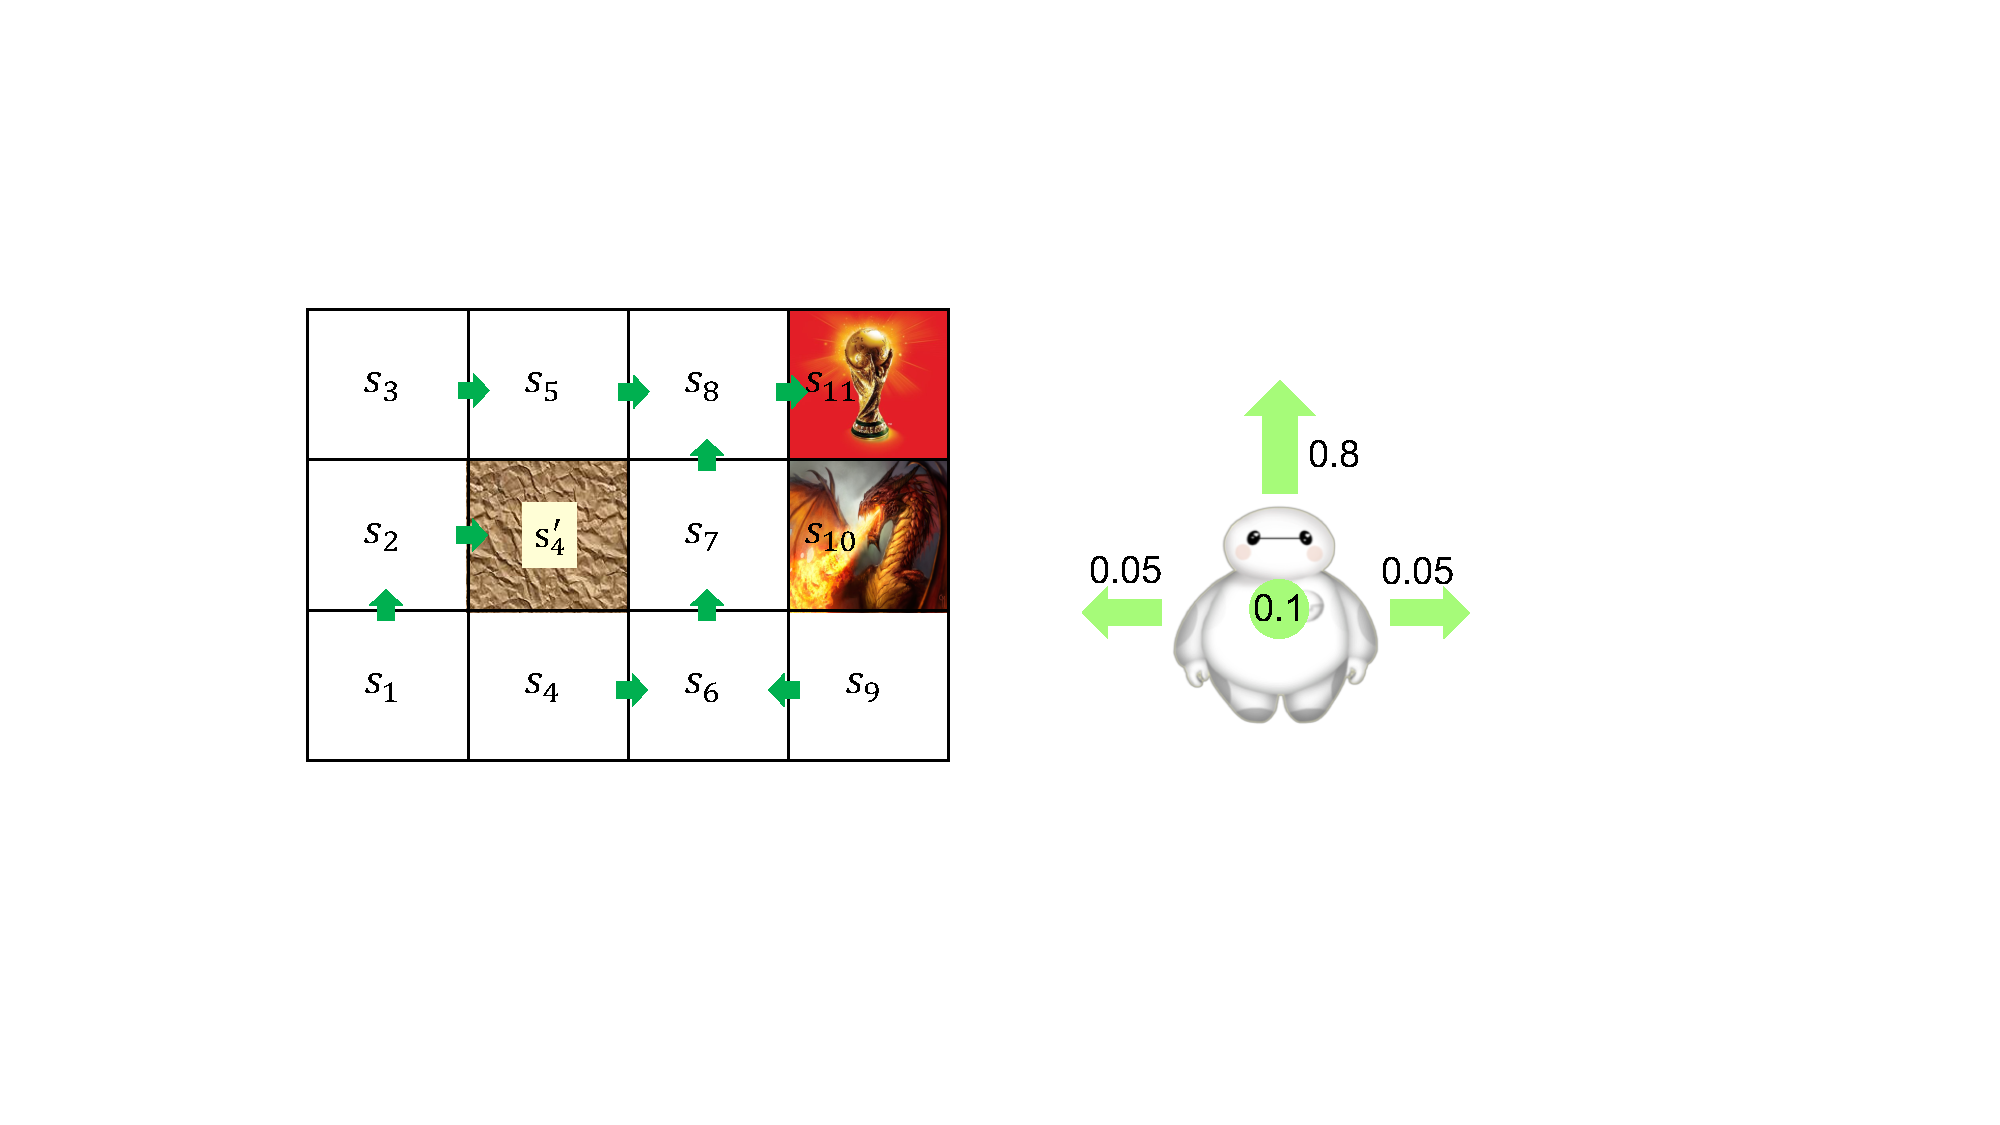
\includegraphics[width=.8\textwidth]{images/Grid_World}
	\caption{Illustration of a grid world with a policy.}\label{fig:gridworld}
\end{figure}


\begin{solution}
	\begin{enumerate}
		\item $$\mathbf{M}=\begin{pmatrix}
				      %   & s1   & s2   & s3   & s4  & s5  & s6   & s7   & s8   & s9   & s10 & s11 \\
				      0.15 & 0.05 & 0    & 0   & 0   & 0    & 0    & 0    & 0    & 0 & 0 \\
				      0.8  & 0.9  & 0.05 & 0   & 0   & 0    & 0    & 0    & 0    & 0 & 0 \\
				      0    & 0.05 & 0.15 & 0   & 0   & 0    & 0    & 0    & 0    & 0 & 0 \\
				      0.05 & 0    & 0    & 0.2 & 0   & 0.05 & 0    & 0    & 0    & 0 & 0 \\
				      0    & 0    & 0.8  & 0   & 0.2 & 0    & 0    & 0    & 0    & 0 & 0 \\
				      0    & 0    & 0    & 0.8 & 0   & 0.1  & 0    & 0    & 0.8  & 0 & 0 \\
				      0    & 0    & 0    & 0   & 0   & 0.8  & 0.15 & 0.05 & 0    & 0 & 0 \\
				      0    & 0    & 0    & 0   & 0.8 & 0    & 0.8  & 0.15 & 0    & 0 & 0 \\
				      0    & 0    & 0    & 0   & 0   & 0.05 & 0    & 0    & 0.15 & 0 & 0 \\
				      0    & 0    & 0    & 0   & 0   & 0    & 0.05 & 0    & 0.05 & 1 & 0 \\
				      0    & 0    & 0    & 0   & 0   & 0    & 0    & 0.8  & 0    & 0 & 1 \\
			      \end{pmatrix}$$
		\item 设 $\mathbf{Q}_t\in\mathbb{R}^{11\times 1}$, $Q_{t,j}=\mathbf{P}(S_t=s_j)$.
		      \begin{enumerate}
			      \item $$\mathbf{Q}_0=\begin{pmatrix}
					            1/11 \\ \vdots \\ 1/11
				            \end{pmatrix}$$
			            $$\mathbf{Q}_1=\mathbf{M}\mathbf{Q}_0=\begin{pmatrix}
					            0.01818182 \\
					            0.15909091 \\
					            0.01818182 \\
					            0.02727273 \\
					            0.09090909 \\
					            0.15454545 \\
					            0.09090909 \\
					            0.15909091 \\
					            0.01818182 \\
					            0.1        \\
					            0.16363636
				            \end{pmatrix}, \mathbf{Q}_2=\mathbf{M}\mathbf{Q}_1=\begin{pmatrix}
					            0.01068182 \\
					            0.15863636 \\
					            0.01068182 \\
					            0.01409091 \\
					            0.03272727 \\
					            0.05181818 \\
					            0.14522727 \\
					            0.16931818 \\
					            0.01045455 \\
					            0.10545455 \\
					            0.29090909
				            \end{pmatrix}$$
			      \item 收敛时有 $\mathbf{M}\mathbf{Q}_\infty=\mathbf{Q}_\infty$, 即 $\mathbf{Q}_\infty$ 是 $\mathbf{M}$ 的特征值为 $1$ 的特征向量。\\
			            经计算,$\mathbf{M}$ 的特征值为 $1$ 的特征向量有
			            $$\mathbf{x}_1=\begin{pmatrix}
					            0 \\ \vdots\\0\\1\\0
				            \end{pmatrix}, \mathbf{x}_1=\begin{pmatrix}
					            0 \\ \vdots\\0\\0\\1
				            \end{pmatrix}$$
			            其任意线性组合都是可能的 $\mathbf{Q}_\infty$, 但
			            $$Q_{\infty,j}=0, j=1,\cdots,9$$
			            所以 $$\lim_{t\rightarrow\infty} \mathbf{P}(S_t=s_i)=0,i=1,\cdots,9$$
			      \item 设 $\mathbf{M}$ 的特征值为 $\lambda_1,\cdots,\lambda_{11}$, 对应的特征向量为 $\mathbf{x}_1,\cdots,\mathbf{x}_{11}$. 设
			            $$\mathbf{X}=\begin{pmatrix}
					            \mathbf{x}_1 & \cdots & \mathbf{x}_{11}
				            \end{pmatrix}$$
			            将 $\mathbf{Q}_0$ 按特征向量构成的基进行分解
			            $$\mathbf{Q}_0=\mathbf{X}\mathbf{a}=\mathbf{X}\begin{pmatrix}
					            a_1 \\ \vdots \\ a_{11}
				            \end{pmatrix}$$
			            则
			            $$\mathbf{M}^t \mathbf{Q}_0=\mathbf{X}\begin{pmatrix}
					            \lambda_1^t a_1 \\ \vdots \\ \lambda_{11}^t a_{11}
				            \end{pmatrix}$$
			            显然只有 $|\lambda|=1$ 才会使 $t\rightarrow\infty$ 对应的分量不为 $0$ 也不发散.\\
			            经计算所有特征值为 $$\mathbf{\lambda=\begin{pmatrix}
						            0.95293107 \\ -0.14865804\\ -0.05      \\0.42423912 \\
						            0.35       \\  0.09706893\\  0.2      \\  0.15      \\
						            0.17441892 \\1\\1
					            \end{pmatrix}}$$
			            由上题可得,$\mathbf{M}$ 有两个特征值为 $1$. 令
			            $$\lambda_{10}=\lambda_{11}=1$$
			            不妨设
			            $$\mathbf{x}_{10}=\begin{pmatrix}
					            0 \\ \vdots\\0\\1\\0
				            \end{pmatrix}, \mathbf{x}_{11}=\begin{pmatrix}
					            0 \\ \vdots\\0\\0\\1
				            \end{pmatrix}$$
			            如此 $\mathbf{X}\mathbf{a}=\mathbf{Q}_0$ 得到的解中
			            $$\begin{aligned}
					            a_{10} & =0.122146474 \\
					            a_{11} & =0.877853526
				            \end{aligned}$$
			            由
			            $$\mathbf{M}^t \mathbf{Q}_0=\mathbf{X}\begin{pmatrix}
					            \lambda_1^t a_1 \\ \vdots \\ \lambda_{11}^t a_{11}
				            \end{pmatrix}$$
			            可知虽然 $\mathbf{X}$ 的不同取值会影响到 $\mathbf{a}$ 的取值,但最后计算的 $\mathbf{M}^t \mathbf{Q}_0$ 却始终是一致的,因而上面的 “不妨设” 是有依据的。\\
			            最后算得
			            $$\begin{aligned}
					            \lim_{t\rightarrow\infty}\mathbf{P}(S_t=s_{10}) & = 0.122146474 \\
					            \lim_{t\rightarrow\infty}\mathbf{P}(S_t=s_{11}) & = 0.877853526
				            \end{aligned}$$
		      \end{enumerate}
		\item $$\mathbf{R}=\begin{pmatrix}
				      0 & 0 & 0 & 0 &  & 0 & -5 & 80 & -5 & 0 & 0
			      \end{pmatrix}^\top$$
		      $$\mathbf{V}^\pi
			      =(\mathbf{I}-\gamma \mathbf{M}^\top) \mathbf{R}
			      =\begin{pmatrix}
				      21.21520135 \\
				      21.97474701 \\
				      71.56706381 \\
				      56.20736261 \\
				      84.60645358 \\
				      64.01394075 \\
				      74.42461495 \\
				      96.35734991 \\
				      47.50293334 \\
				      0           \\
				      0
			      \end{pmatrix}
		      $$
		\item 以上 (2b) 的证明即是与 $\mathbf{P}(S_0=s_i)$ 无关的,只与 $\mathbf{M}$ 相关,此处不再重复。
	\end{enumerate}
\end{solution}


\newpage
\begin{exercise}[Optimal Policy \textnormal{40pts}]
	Consider the grid world problem described in Exercise \ref{exercise:GridWorld}. Let $\pi^*$ be the optimal policy, $V^*$ the corresonding value function, and $\gamma=0.9$.

	\begin{enumerate}
		\item (10pts) Please derive the Bellman Equation in terms of the value function $V^*$ and the $Q$ function, respectively.

		\item (10pts) Please choose one of the algorithms we introduced in class to find $\pi^*$ and $V^*$ respectively and write their pseudocode (hand in your code if you have one).

		\item (20pts) Please design a reward scheme such that following the resulting optimal policy will never lose. Specifically, you need to derive the resulting optimal policy and show  $$\lim_{t\rightarrow\infty}\mathbf{P}(S_t=s_i)=0,\,i=1,\ldots,10,$$
		      whenever $\mathbf{P}(S_0=s_{10})=\mathbf{P}(S_0=s_{11})=0$.
		      %for any $\mathbf{P}(S_0=s_i)$, $i=1,\ldots,9$, and $\mathbf{P}(S_0=s_{10})=\mathbf{P}(S_0=s_{11})=0$.
	\end{enumerate}


\end{exercise}

\begin{solution}
	\begin{enumerate}
		\item  从状态 $s_t$ 开始时,期望累计奖励值为
		      $$V^\pi(s_t)=\expect{\sum_{i=0}^{\infty} \gamma^i R_{t+i} \mid S_t=s_t}$$
		      所以有
		      $$V^\pi(s)=\expect{r(s,\pi(s))}+\gamma \sum_{s'} P(s'\mid s, \pi(s))V^\pi (s')$$
		      设 $\mathbf{T}$ 为概率转移矩阵,$t_{ij}=P(S_{t+1}=s_j \mid S_t=s_i)$. 上式表示为
		      $$\mathbf{V}=\mathbf{R}+\gamma \mathbf{T}\mathbf{V}$$
		      所以也有
		      $$\mathbf{V}^*=\mathbf{R}+\gamma \mathbf{T}\mathbf{V}^*$$
		      即 $$\mathbf{V}^*=\max_{\mathbf{R},\mathbf{T}}(\mathbf{I}-\gamma \mathbf{T})^{-1}\mathbf{R}$$
		      定义
		      $$Q(s,a)=\expect{r(s,a)}+\gamma\sum_{s'}P(s'\mid s,a)V^*(s')$$
		      显然有 $$\pi^*(s)=\argmax_a Q(s,a)$$
		      由 $V$ 的 Bellman 方程可知
		      $$V^*(s)=\max_a Q(s,a)$$
		      所以可知
		      $$Q(s,a)=\expect{r(s,a)}+\gamma \sum_{s'}P(s'\mid s,a)\max_{a'}Q(s',a')$$
		\item 见下文 Algorithm \ref{alg:value_iteration}.
		\item 将到达 $s_{10}$ 的奖励设置为 $-\infty$, 其余不变。\\
		      仍然采用 Value Iteration 的方法求最优解,值得注意的是,在迭代中,有
		      $$\begin{aligned}
				        & \expect{r(s_{7},\text{up})}
				      = & \expect{r(s_{7},\text{right})}
				      = & \expect{r(s_{7},\text{down})}  \\
				      = & \expect{r(s_{9},\text{up})}
				      = & \expect{r(s_{9},\text{left})}
				      = & \expect{r(s_{9},\text{right})} \\
				      = & -\infty
			      \end{aligned}$$
		      所以 $\pi(s_7)$ 必然为 left, $\pi(s_9)$ 必然为 down.\\
		      最后得到的最优 $\pi^*$ 为
		      $$\begin{aligned}
				      \pi(s_1) = \text{up}\ \
				       & \pi(s_2) = \text{up}\ \
				       & \pi(s_3) = \text{right}\ \
				       & \pi(s_4) = \text{left}\ \
				       & \pi(s_5) = \text{right}\  \ \\
				      \pi(s_6) = \text{left}\ \
				       & \pi(s_7) = \text{left}\ \
				       & \pi(s_8) = \text{right}\ \
				       & \pi(s_9) = \text{down}\ \
			      \end{aligned}$$
		      对应的
		      $$\mathbf{M}=\begin{pmatrix}
				      %   & s1   & s2   & s3   & s4  & s5  & s6   & s7   & s8   & s9   & s10 & s11 \\
				      0.15 & 0   & 0    & 0.8 & 0   & 0    & 0    & 0    & 0    & 0 & 0 \\
				      0.8  & 0.2 & 0.05 & 0   & 0   & 0    & 0    & 0    & 0    & 0 & 0 \\
				      0    & 0.8 & 0.15 & 0   & 0   & 0    & 0    & 0    & 0    & 0 & 0 \\
				      0.05 & 0   & 0    & 0.2 & 0   & 0.8  & 0    & 0    & 0    & 0 & 0 \\
				      0    & 0   & 0.8  & 0   & 0.2 & 0    & 0    & 0    & 0    & 0 & 0 \\
				      0    & 0   & 0    & 0   & 0   & 0.15 & 0.05 & 0    & 0.05 & 0 & 0 \\
				      0    & 0   & 0    & 0   & 0   & 0.05 & 0.9  & 0.05 & 0    & 0 & 0 \\
				      0    & 0   & 0    & 0   & 0.8 & 0    & 0.05 & 0.15 & 0    & 0 & 0 \\
				      0    & 0   & 0    & 0   & 0   & 0    & 0    & 0    & 0.95 & 0 & 0 \\
				      0    & 0   & 0    & 0   & 0   & 0    & 0    & 0    & 0    & 1 & 0 \\
				      0    & 0   & 0    & 0   & 0   & 0    & 0    & 0.8  & 0    & 0 & 1 \\
			      \end{pmatrix}$$
		      和第 3 题的情况一样,$\mathbf{M}$ 的特征值只有两个为 $1$, 且对应的特征向量为
		      $$\mathbf{x}_1=\begin{pmatrix}
				      0 \\ \vdots\\0\\1\\0
			      \end{pmatrix}, \mathbf{x}_1=\begin{pmatrix}
				      0 \\ \vdots\\0\\0\\1
			      \end{pmatrix}$$
		      其任意线性组合都是可能的 $\mathbf{Q}_\infty$, 但
		      $$Q_{\infty,j}=0, j=1,\cdots,9$$
		      所以 $$\lim_{t\rightarrow\infty} \mathbf{P}(S_t=s_i)=0,i=1,\cdots,9$$
		      又因为 $\mathbf{P}(S_0=s_{10})=0$, 所以 $Q_{\infty,10}=0$, 所以
		      $$\lim_{t\rightarrow\infty} \mathbf{P}(S_t=s_{10})=0$$
	\end{enumerate}
\end{solution}

\begin{algorithm}
	\caption{Get $V^*$ and $\pi^*$ by Value Iteration}
	\label{alg:value_iteration}
	\textbf{Input:} 状态集 $\mathcal{S}$, 动作集 $\mathcal{A}$, 每个状态以及与其对应的动作决定的奖励 $r(s,a)$ 和状态转移概率 $P(s'\mid s,a)$ \\
	\textbf{Output:}  $\mathbf{V}^*$ 和 $\mathbf{\pi}^*$
	\begin{algorithmic}[1]
		\STATE 对 $\forall s\in \mathcal{S}$, 设置 $V(s)$ 为任意取值
		\STATE 对 $\forall s\in \mathcal{S}$, 设置 $V'(s)$ 为任意不为 $V(s)$ 的值
		\STATE 对 $\forall s\in \mathcal{S}$, 设置 $\pi(s)$ 为 $\mathcal{A}$ 中任意取值

		\WHILE{$\exists s\in\mathcal{S}, V(s)\neq V'(s)$}
		\FOR{$\forall s\in\mathcal{S}$}
		\FOR{$\forall a\in\mathcal{A}$}
		\STATE $Q(s,a)\leftarrow \expect{r(s,a)}+\gamma \sum_{s'}P(s'\mid s,a)V(s')$
		\ENDFOR
		\STATE $V'(s)\leftarrow V(s)$
		\STATE $\pi(s)\leftarrow \argmax_a Q(s,a)$
		\STATE $V(s)\leftarrow Q(s,\pi(s))$
		\ENDFOR
		\ENDWHILE
		\RETURN $\mathbf{V}, \mathbf{\pi}$
	\end{algorithmic}
\end{algorithm}

\newpage
\begin{exercise}[Policy Iteration \textnormal{20pts}]
	Consider a Markov Decision Process with bounded rewards and finite state-action pairs. The transition probability is $\mathbf{P}[s'|s,a]$ and the reward function is $r(s,a)$. Let $\pi:\mathcal{S}\rightarrow\mathcal{A}$ be a deterministic policy.
	\begin{enumerate}
		\item (10pts) Let $Q^\pi (s,a)$ be the accumulated reward by performing the action $a$ first and then following the policy $\pi$. Find the Bellman Equation for $Q^\pi$.
		\item (10pts) Consider a new policy $\pi'$ given by
		      \begin{align*}
			      \pi'(s)=\argmax_{a\in\mathcal{A}} Q^\pi(s,a).
		      \end{align*}
		      Note that if $\argmax_{a\in\mathcal{A}} Q^\pi(s,a)$ is not unique, we can choose one action arbitrarily. Show that  $V^{\pi'}(s) \geq V^\pi(s)$ for all $s\in \mathcal{S}$.
	\end{enumerate}
\end{exercise}

\begin{solution}
	\begin{enumerate}
		\item 由定义可知
		      $$Q^\pi(s,a)=\expect{r(s,a)}+\gamma \sum_{s'} P(s'\mid s,a)V^\pi(s')$$
		      而
		      $$Q^\pi(s,\pi(s))=V^\pi(s)$$
		      所以
		      $$Q^\pi(s,a)=\expect{r(s,a)}+\gamma \sum_{s'} P(s'\mid s,a)Q^\pi(s',\pi(s'))$$
		\item 逐级展开
		      $$\begin{aligned}
				      V^\pi(s)
				       & =Q^\pi(s,\pi(s))                                                                                                                                       \\
				       & \leq Q^\pi(s,\pi'(s))                                                                                                                                  \\
				       & = \expect{r(s,\pi'(s))}+\gamma \sum_{s'} P(s'\mid s,\pi'(s))V^\pi(s')                                                                                  \\
				       & \leq \expect{r(s,\pi'(s))}+\gamma \sum_{s'} P(s'\mid s,\pi'(s))Q^\pi(s',\pi'(s'))                                                                      \\
				       & = \expect{r(s,\pi'(s))}+\gamma \sum_{s'} P(s'\mid s,\pi'(s)) \left( \expect{r(s',\pi'(s'))}+\gamma \sum_{s''} P(s''\mid s',\pi'(s'))V^\pi(s'') \right) \\
				       & \leq \cdots                                                                                                                                            \\
				       & = V^{\pi'}(s)
			      \end{aligned}$$
	\end{enumerate}
\end{solution}



%\newpage
% \bibliography{refs}
%\bibliographystyle{abbrv}

%%%%%%%%%%%%%%%%%%%%%%%%%%%%%%%%%%%%%%%%%%%%%%%%%%%%%%%%%%%%%%%%

\end{document}
